\section{Parcelamiento del \'area de Broca}
\label{sec:parcela_broca}

Decidimos comenzar parcelando solo el \'area de Broca. El ser una regi\'on
chica permite generar resultados en poco tiempo y comparar de manera
visual los m\'etodos implementados. Situamos semillas a $3mm$ de la
corteza siguiendo la secci\'on \ref{sec:semillas} y generamos tractogramas
utilizando el algoritmo \ref{alg:itract} de la secci\'on 
\label{sec:convergencia}. En total se crearon aproximadamente $760$
semillas con sus tractogramas. A continuaci\'on mostramos distintas
parcelaciones de la corteza obtenidas mediante el m\'etodo de 
Moreno-Dominguez y el nuestro. \\

\subsection{M\'etodo Moreno-Dominguez}
\label{sec:moreno_broca}

Parcelamos el \'area de Broca usando el m\'etodo de Moreno-Dominguez. Al
igual que en la secci\'on \label{sec:clustering_moreno}, descartamos los
tractogramas con un solo voxel visitado y aplicamos un $threshold$ de $0.4$
en cada voxels. Las figuras \ref{fig:moreno0} y \ref{fig:moreno1} se 
generaron sin aplicar restricciones en ninguna iteraci\'on del $clustering$
($k=0$). Ambas muestran el resultado obtenido de un mismo dendrograma
cortado a distintos niveles de profundidad. La figura \ref{fig:moreno2}
muestra los resultados usando $k=400$. Esto es, las primeras $400$
uniones son solo entre $clusters$ vecinos y de tama\~no homog\'eneo. La
figura \ref{fig:moreno3} muestra la parcelaci\'on obtenida usando $k=700$.
\\

\begin{figure}[h!]
    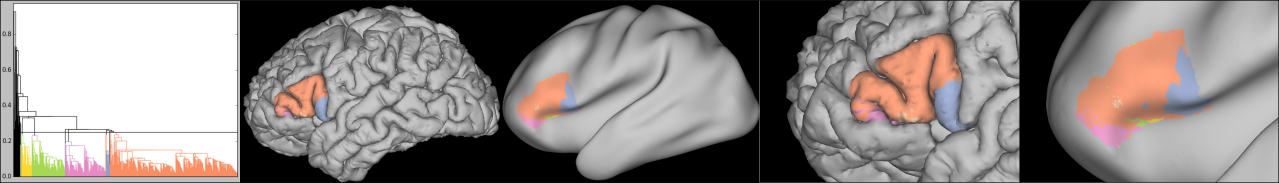
\includegraphics[width=\textwidth]{img/broca/moreno_0.png}
    \caption{Parcelamiento del \'area de Broca utilizando el m\'etodo de 
             Moreno-Dominguez sin aplicar restricciones en ninguna
             iteraci\'on.}
    \label{fig:moreno0}
\end{figure}
                                                                                                                       
\begin{figure}[h!]
    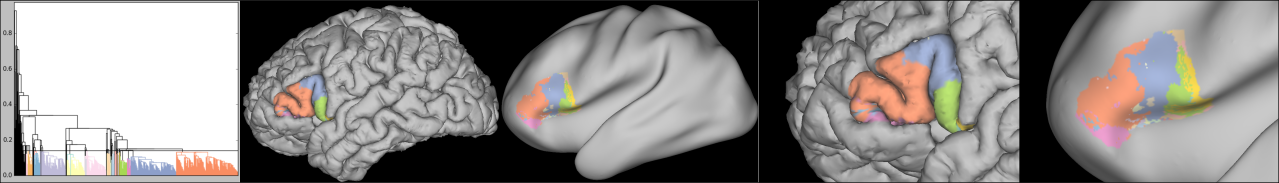
\includegraphics[width=\textwidth]{img/broca/moreno_0_deep.png}
    \caption{Parcelamiento del \'area de Broca utilizando el m\'etodo de 
             Moreno-Dominguez sin aplicar restricciones en ninguna
             iteraci\'on. Corte con mayor profundidad en el dendrograma.}
    \label{fig:moreno1}
\end{figure}

\begin{figure}[h!]
    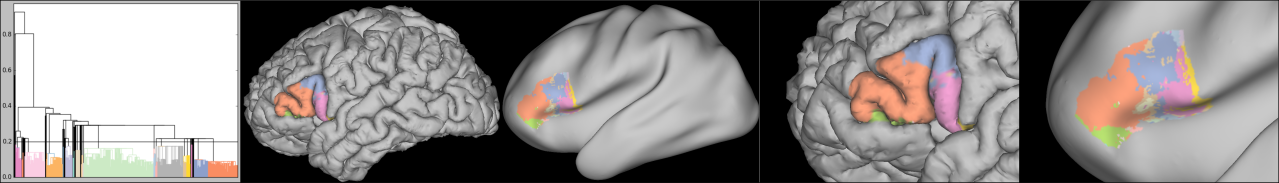
\includegraphics[width=\textwidth]{img/broca/moreno_400.png}
    \caption{Parcelamiento del \'area de Broca utilizando el m\'etodo de 
             Moreno-Dominguez. Las primeras 400 uniones fueron entre
             $clusters$ vecinos.}
    \label{fig:moreno2}
\end{figure}

\begin{figure}[h!]
    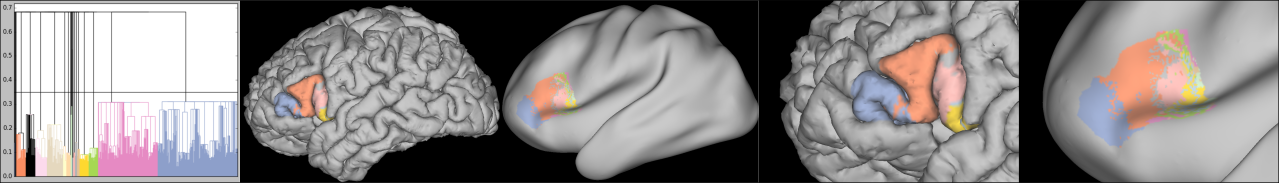
\includegraphics[width=\textwidth]{img/broca/moreno_750.png}
    \caption{Parcelamiento del \'area de Broca utilizando el m\'etodo de 
             Moreno-Dominguez. Las primeras 700 uniones fueron entre
             $clusters$ vecinos.}
    \label{fig:moreno3}
\end{figure}


\subsection{Parcelamiento en el espacio $LogOdds$}
\label{sec:nuestro_broca}

Parcelamos el \'area de Broca usando nuestro m\'etodo. Al igual que en la 
secci\'on \label{ch:nuestro}, descartamos los tractogramas con un solo
voxel visitado y aplicamos un $threshold$ de $0.25$ en cada voxels. 
Las figuras \ref{fig:nuestro0} y \ref{fig:nuestro0} se generaron sin 
aplicar restricciones en ninguna iteraci\'on del $clustering$ ($k=0$).
Ambas muestran el resultado obtenido de un mismo dendrograma cortado a 
distintos niveles de profundidad. La figura \ref{fig:nuestro2} muestra los
resultados usando $k=400$. Esto es, las primeras $400$ uniones son
solo entre $clusters$ vecinos y de tama\~no homog\'eneo. La figura
\ref{fig:nuestro3} muestra la parcelaci\'on obtenida usando $k=700$.\\

\begin{figure}[h!]
    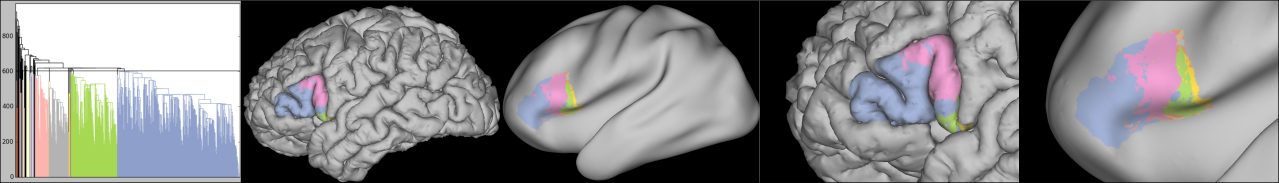
\includegraphics[width=\textwidth]{img/broca/logit_0.png}
    \caption{Parcelamiento del \'area de Broca utilizando nuestro m\'etodo 
             sin aplicar restricciones en ninguna iteraci\'on.}
    \label{fig:nuestro0}
\end{figure}
                                                                                                                        
\begin{figure}[h!]
    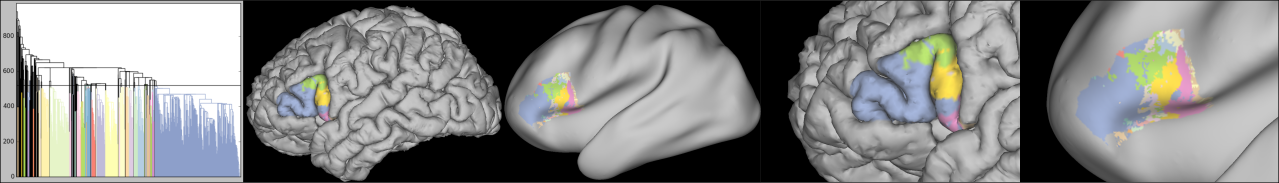
\includegraphics[width=\textwidth]{img/broca/logit_0_deep.png}
    \caption{Parcelamiento del \'area de Broca utilizando nuestro m\'etodo
             sin aplicar restricciones en ninguna iteraci\'on. Corte con
             mayor profundidad en el dendrograma.}
    \label{fig:nuestro1}
\end{figure}

\begin{figure}[h!]
    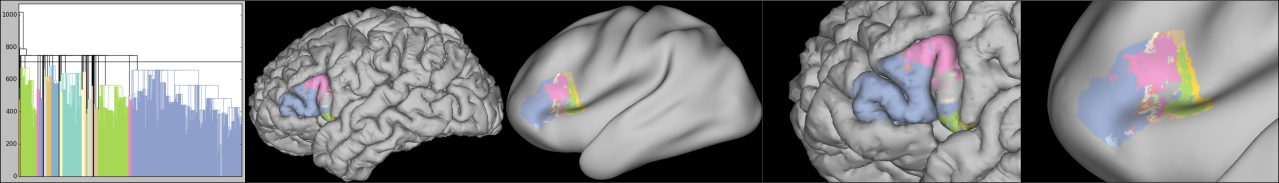
\includegraphics[width=\textwidth]{img/broca/logit_400.png}
    \caption{Parcelamiento del \'area de Broca utilizando nuestro m\'etodo.
             Las primeras 400 uniones fueron entre $clusters$
             vecinos.}    
    \label{fig:nuestro2}
\end{figure}

\begin{figure}[h!]
    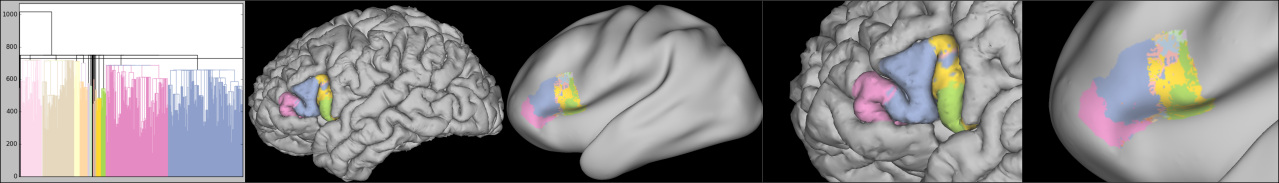
\includegraphics[width=\textwidth]{img/broca/logit_750.png}
    \caption{Parcelamiento del \'area de Broca utilizando nuestro m\'etodo.
             Las primeras 700 uniones fueron entre $clusters$
             vecinos.}       
    \label{fig:nuestro3}
\end{figure}

\subsection{Resultados de los m\'etodos en mayor detalle}
\label{sec:acercamiento}

Para facilitar una primera comparaci\'on visual entre los m\'etodos 
presentamos las parcelaciones con mayor detalle. Las figuras 
\ref{fig:ambos0}; \ref{fig:ambos1} y \ref{fig:ambos2} presentan
parcelaciones obtenidas usando $k=0$, $k=400$ y $k=700$ respectivamente.
Esto es: el algoritmo sin restricciones; las primeras $400$ uniones entre
$clusters$ vecinos y las primeras $700$ uniones entre $clusters$ vecinos
respectivamente.
En cada figura se puede apreciar una parcelaci\'on obtenida con el 
m\'etodo Moreno-Dominguez a la izquierda y una parcelaci\'on obtenida 
con nuestro m\'etodo a la derecha. Los dendrogramas no se presentan, dada
la diferencia de alturas y cortes no aportan a la comparaci\'on visual. \\

\begin{figure}[h!]
    \centering
    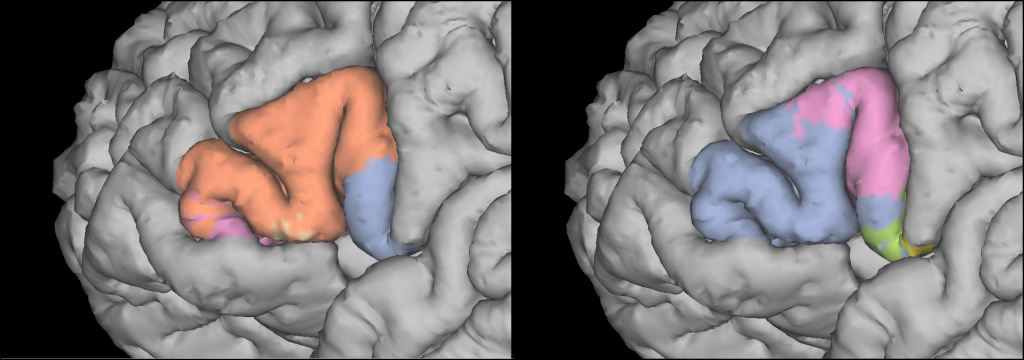
\includegraphics[width=\textwidth]{img/broca/vs_0.png}
    \caption{Detalle sobre las parcelas obtenidos utilizando 
             el m\'etodo de Moreno-Dominguez (izquierda) y el nuestro
             (derecha). No se aplicaron restricciones en las iteraciones.}
    \label{fig:ambos0}
\end{figure}

\begin{figure}[h!]
    \centering
    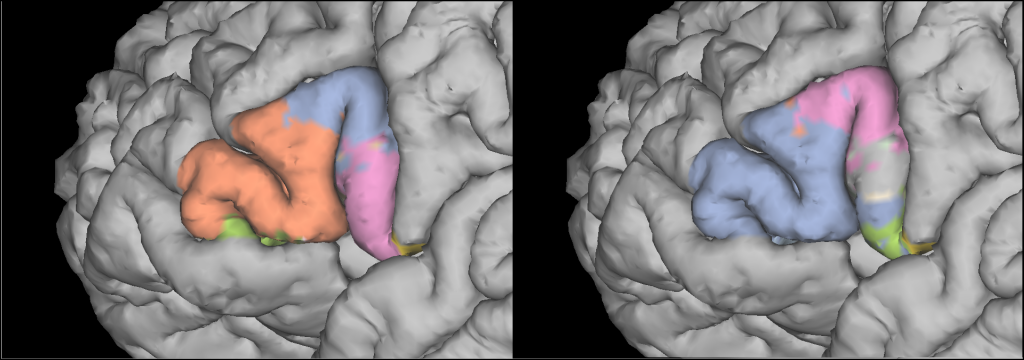
\includegraphics[width=\textwidth]{img/broca/vs_400.png}
    \caption{Detalle sobre las parcelas obtenidos utilizando 
             el m\'etodo de Moreno-Dominguez (izquierda) y el nuestro
             (derecha). Las primeras 400 uniones fueron entre
             $clusters$ vecinos.}
    \label{fig:ambos1}    
\end{figure}
    
\begin{figure}[h!]
    \centering
    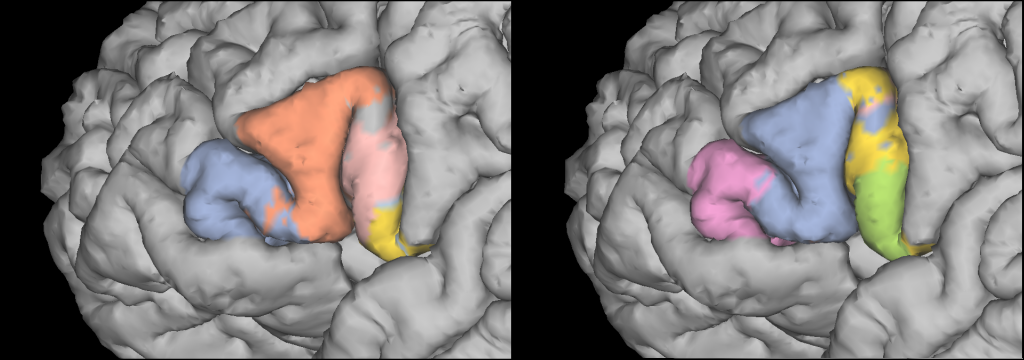
\includegraphics[width=\textwidth]{img/broca/vs_700.png}
    \caption{Detalle sobre las parcelas obtenidos utilizando 
             el m\'etodo de Moreno-Dominguez (izquierda) y el nuestro
             (derecha). Las primeras 700 uniones fueron entre 
             $clusters$ vecinos.}
    \label{fig:ambos2}
\end{figure}

